%---------------------------------------------------------------------
% Course 	: Introduction To web sciences
% Professor : Dr.Nelson
% Name   	: Babitha Bokka
% Assignment: 3
%---------------------------------------------------------------------
\documentclass[12pt]{article}
%--------------------------------------------------------------------
% packages required
%--------------------------------------------------------------------
\usepackage{graphicx}
\usepackage{listings}
\usepackage{hyperref}
\usepackage{caption}
\usepackage{color}
\graphicspath{ {images/} }
%--------------------------------------------------------------------
% Start Margins
%--------------------------------------------------------------------
\addtolength{\oddsidemargin}{-.875in}
\addtolength{\evensidemargin}{-.875in}
\addtolength{\textwidth}{1.75in}
\addtolength{\topmargin}{-.885in}
\addtolength{\textheight}{1.95in}
%-------------------------------------------------------------------
% End Margins
%--------------------------------------------------------------------
\definecolor{codegreen}{rgb}{0,0.6,0}
\definecolor{codegray}{rgb}{0.5,0.5,0.5}
\definecolor{codepurple}{rgb}{0.58,0,0.82}
\definecolor{backcolour}{rgb}{0.95,0.95,0.92}
 
\lstdefinestyle{mystyle}{
    backgroundcolor=\color{backcolour},   
    commentstyle=\color{codegreen},
    keywordstyle=\color{magenta},
    numberstyle=\tiny\color{codegray},
    stringstyle=\color{codepurple},
    basicstyle=\footnotesize,
    breakatwhitespace=false,         
    breaklines=true,                 
    captionpos=b,                    
    keepspaces=true,                 
    numbers=left,                    
    numbersep=5pt,                  
    showspaces=false,                
    showstringspaces=false,
    showtabs=false,                  
    tabsize=2
}
 
\lstset{style=mystyle}

\begin{document}

%---------------------------------------------------------------------
%Making the title page
%---------------------------------------------------------------------
\begin{titlepage}
\title{INTRODUCTION TO WEB SCIENCES:\\*Assignment 3}
\author{Babitha Bokka}
\date{3 october 2014}
\maketitle
\end{titlepage}

%---------------------------------------------------------------------
%Table of contents
%---------------------------------------------------------------------
\tableofcontents
\newpage
%------------------------------------------------------------------
%Question 1
%------------------------------------------------------------------
\section{Question 1}

Download HTML content of 1000 URIs extracted in assignment #2.
\subsection{Approach Towards the Solution}
There are many good ways to extract the HTML from a URL. I approached the problem byt using requests, urllib2 and curl but among all of the three i observed curl command has extrected more of html from the URIs.
\begin{enumerate}
	\item Requests and urllib2 library in python.
	\item curl 
\end{enumerate}
\subsubsection{Desciption of extractHtml.sh}
\begin{enumerate}
	\item 
	\item 
	\item 
	\item 
	\item 
	\item 
\end{enumerate}
\subsubsection{Desciption of scrapeHtml.sh}
\begin{enumerate}
	\item 
	\item 
	\item 
	\item 
	\item 
\end{enumerate}
\newpage
\subsection{Source Code}
\subsubsection{extractHtml.sh}
\lstinputlisting[breaklines=True,language=Python]{../Q1/extractHtml.sh}
\subsubsection{scrapeHtml.sh}
\lstinputlisting[breaklines=True,language=Python]{../Q1/scrapeHtml.sh}
\subsubsection{requestsExtractHtml.py}
\subsubsection{urllibExtractHtml.py}
\newpage
\subsection{InputFile : uniqueUri.txt}
The input is taken from the assignment #2 , the 1000 unique URIs.
\lstinputlisting[breaklines=True]{../Q1/uniqueUri.txt}
\newpage
\subsection{OutputFiles}
A sample of raw and processed HTML files
\subsubsection{.txt}
\lstinputlisting[breaklines=True]{../Q1/.txt}

%------------------------------------------------------------------
%Question 2
%------------------------------------------------------------------
\newpage
\section{Question 2}

To extract the timemaps of the 1000 unique URLs extracted obtained in Question 1 and count the number of mementos for each URL. Each memento represents a date and time where an individual URL was modified.

\subsection{Approach Towards the Solution}
To find the number of mementos, I used regular expressions (regexp) to locate the strings rel="memento" and rel="timemap". Occurances of the string rel="memento" were recorded to obtain a count of mementos for each URL. If there was a line containing rel="timemap", another page of mementos was available. I looped through each momento page until all mementos were counted. I then stored the results (mometo count, URL) in a text file.
\subsubsection{momentoTwitter.py}
\begin{enumerate}
	\item Open finalUniqueUri.txt .
	\item Read each URL.
	\item Append it to http://mementoweb.org/timemap/link/ .
	\item Request the complete URL.
	\item Get the response, and count the number of mementos.
	\item Check if there is a timemap line.
	\item If a timemap line is encountered, loop and collect all  momentos.
	\item Store the results to momentoUri.txt .
\end{enumerate}
\newpage
\subsection{Source Code}
\subsubsection{momentoTwitter.py}
\lstinputlisting[breaklines=True,language=Python]{../Q2/momentoTwitter.py}
\newpage
\subsection{OutputFiles}
\subsubsection{momentoUri.txt}
\lstinputlisting[breaklines=True]{../Q2/momentoForDoc.txt}
\newpage
%------------------------------------------------------------------
% Histogram
%------------------------------------------------------------------
\subsection{Histogram }
\subsubsection{code to generate the Histogram histogramCode.txt}
\lstinputlisting[breaklines=True]{../Q2/histogramCode.txt}
\subsubsection{Description of Histograms}
Figure \ref{fig:initial-histogram} represents mementos vs URI. If you observe the initial histogram, it does not give you a clear picture how many URIs have how many momentos.

The scaled histogram, Figure \ref{fig:scaled-histogram}, provdes additional insight about URIs and respective mementos.

\begin{figure}[ht]
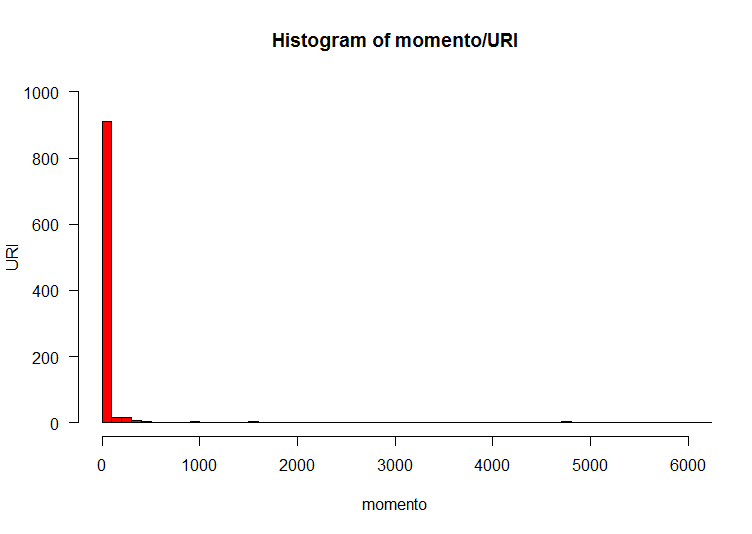
\includegraphics[scale=0.7]{../Q2/histogramMomentoURI_1}
\centering
\caption{Intial-histogram}
\label{fig:initial-histogram}
\end{figure}
\newpage
\begin{figure}[ht]
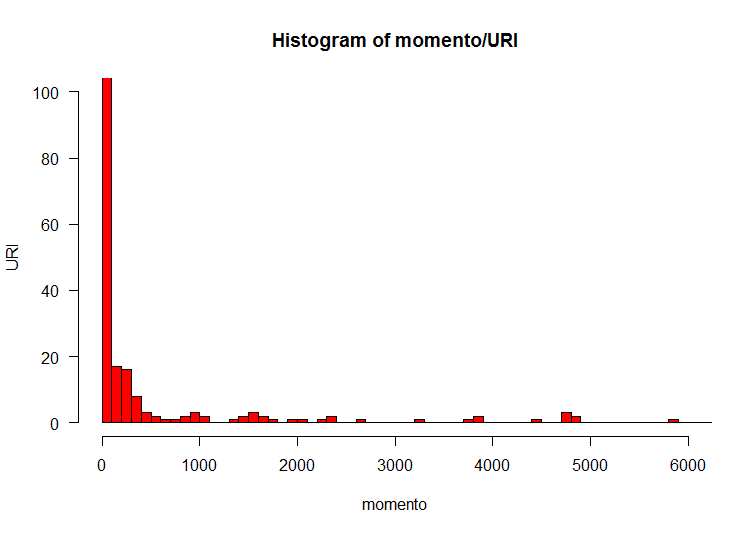
\includegraphics[scale=0.7]{../Q2/histogramMomentoURI_2}
\centering
\caption{Scaled-histogram}
\label{fig:scaled-histogram}
\end{figure}
\newpage
%------------------------------------------------------------------
%Question 3
%------------------------------------------------------------------
\section{Question 3}

Estimate the age of the each unique url by using the carbon date tool.
\subsection{Approach Towards the Solution}

To estimate the carbon date(estimated creation date) of each URL we download the carbondate tool files and run local.py get the creation dates and store them to a carbondateDays.txt.

CarbonDateTwitter.txt has the carbon date and URL, to estimate the age of the each url till today (date it was created and to till date gives us the number of days the url has been created) program daysCountTwitter.py will read each line and parses the date and estimates the number of days.

Relation between the memento and days can be obtained by running momentoDays.py which uses dictionary to store all the days and URL from carbonDateDays.txt for each URL it reads momentoUri.txt and checks whether there is a URL with greater than 0 momentos if it encounters any of the URL then that memento is appended to the dictionary.Then the results(days--momento) are stored in momentoDays.txt .
\subsubsection{description of daysCountTwitter.py}
\begin{enumerate}
	\item Modify the local.py extract the dates for each URL.
	\item Store in carbonDateTwitter.txt.
	\item Now load the file in to daysCountTwitter.py.
	\item Program calculates the number of days it has been since the URL has been created .
	\item Store the days and URL into carbonDateDays.txt.	
\end{enumerate}
\subsubsection{description of momentoDays.py}
\begin{enumerate}
	\item Open the file momentoDays.txt.
	\item Store the days and URL into a dictionary with key as URL {key:URL value :list[date]} value as days.	
	\item Now open the momentoUri.txt .
	\item Read each line and compare the URL with the dictionary key URL if there is a match and the number of mementos for that URL is greater that zero store the URL in momentoDays.txt.
	\item momentoDays.txt has days , mementos.
\end{enumerate}

\newpage
\subsubsection{daysCountTwitter.py}
\lstinputlisting[breaklines=True,language=Python]{../Q3/daysCountTwitter.py}
\newpage
\subsubsection{momentoDays.py}
\lstinputlisting[breaklines=True,language=Python]{../Q3/momentoDays.py}
\newpage
\subsection{OutputFiles}
\subsubsection{carbonDateTwitter.txt}
\lstinputlisting[breaklines=True]{../Q3/carbonForDoc.txt}
\subsubsection{carbonDateDays.txt}
\lstinputlisting[breaklines=True]{../Q3/carbonDaysForDoc.txt}
\subsubsection{momentoDays.txt}
\lstinputlisting[breaklines=True]{../Q3/momentoDaysForDoc.txt}
\newpage


\subsection{Scatterplot}
\subsubsection{Code to generate the Scatterplot scatterplotCode.txt}
\lstinputlisting[breaklines=True]{../Q3/scatterplotCode.txt}
\subsubsection{Description of Histogram}
Figure \ref{fig:initial-histogram} brings up the relation between the days and the memento.Figure \ref{fig:initial-histogram} and Figure \ref{fig:scaled-histogram} are plotted on the same data but Figure \ref{fig:scaled-histogram} gives additional insight. 

\begin{figure}[ht]
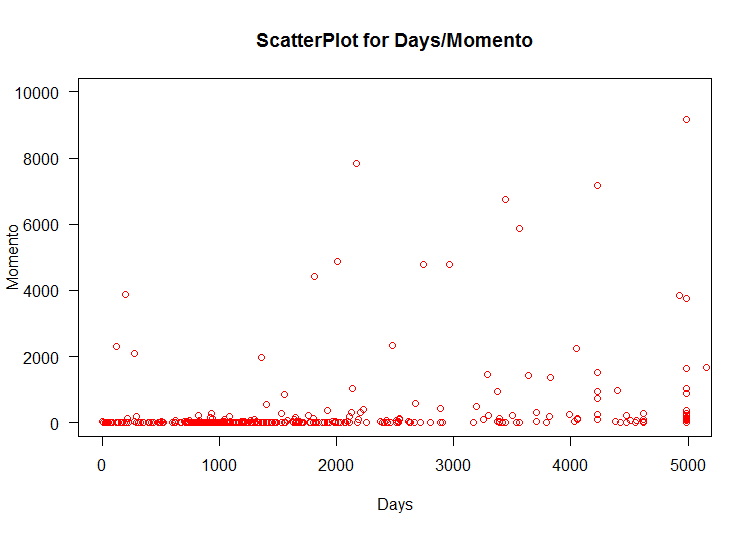
\includegraphics[scale=0.7]{../Q3/scatterDaysMomento_1}
\centering
\caption{intial scatterplot}
\label{intial-scatterplot}
\end{figure}
\newpage

\begin{figure}[ht]
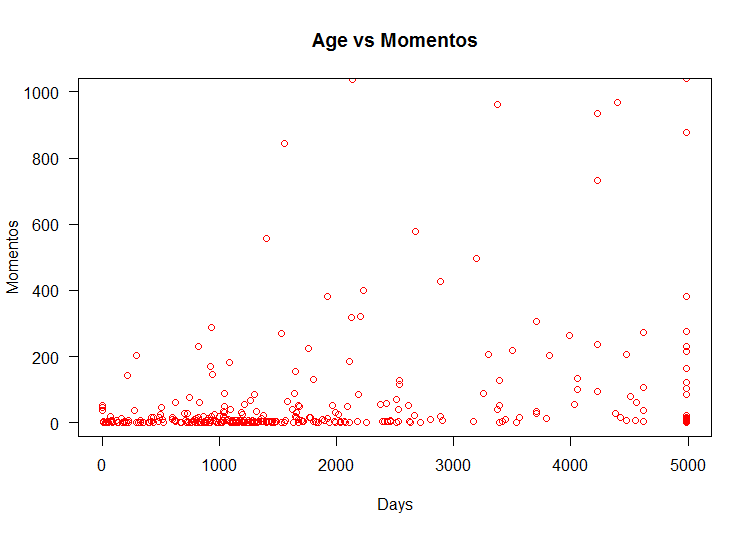
\includegraphics[scale=0.7]{../Q3/scatterDaysMomento_2}
\centering
\caption{Scaled scatterplot}
\label{scaled-scatterplot}
\end{figure}
\newpage
%-------------------------------------------------------------------
%References
%-------------------------------------------------------------------
\bibliographystyle{plain}
\bibliography{A2_report}
\cite{*}
\end{document}